\documentclass[pdf]{beamer}

\usepackage[utf8]{inputenc}
\usepackage[spanish]{babel}

\usepackage{ragged2e} % Paquete para trabajar texto.

\mode<presentation>

\usepackage{lmodern}
\usetheme{Madrid} 

\usepackage{float} %para fijar tablas
\usepackage{multirow} %Para tablas
\usepackage{booktabs}

\usepackage{csvsimple} %csv to table

\usepackage{hyperref}%Links
\hypersetup{  %formato link
    colorlinks=true,
    linkcolor=green,
    filecolor=blue,      
    urlcolor=blue}

% Para evitar errores de compilación en \author
\pdfstringdefDisableCommands{%
  \def\\{}%
  \def\vspace{}%
}

\usepackage{wrapfig} %para acomodar gráficos con texto.
\usepackage{graphicx} % para combinar gráficos con listas
\usepackage{graphbox}   % allows to add keys to \includegraphics
\usepackage{lipsum}     % only for testing purposes

\title[Curso Data Science]{\textbf{Análisis socioeducativo de los habitantes de la Ciudad de Buenos Aires}}

\author[Coderhouse]{\textbf{Profesor:} Damian Dapueto \\ \vspace{0.1cm} \textbf{Tutor:} Héctor Alonso \\ \vspace{0.1cm} \textbf{Grupo de Trabajo:} Lucia Buzzeo, Lucia Hukovsky,\\ Jose Saint German, Juan Martín Carini}

\date{}

\begin{document}
\justifying{ 

\begin{frame}

    \begin{center}
        
\includegraphics[scale=0.2]{../Informe/Imagenes/Coder2.jpg}
    \end{center}

    \titlepage%

\end{frame}

\section{Introducción}

    \subsection{Resumen del proyecto}

\begin{frame}{Introdución}

    % \begin{wrapfigure}{r}[R]{0.5\textwidth}
    %     \centering
    %     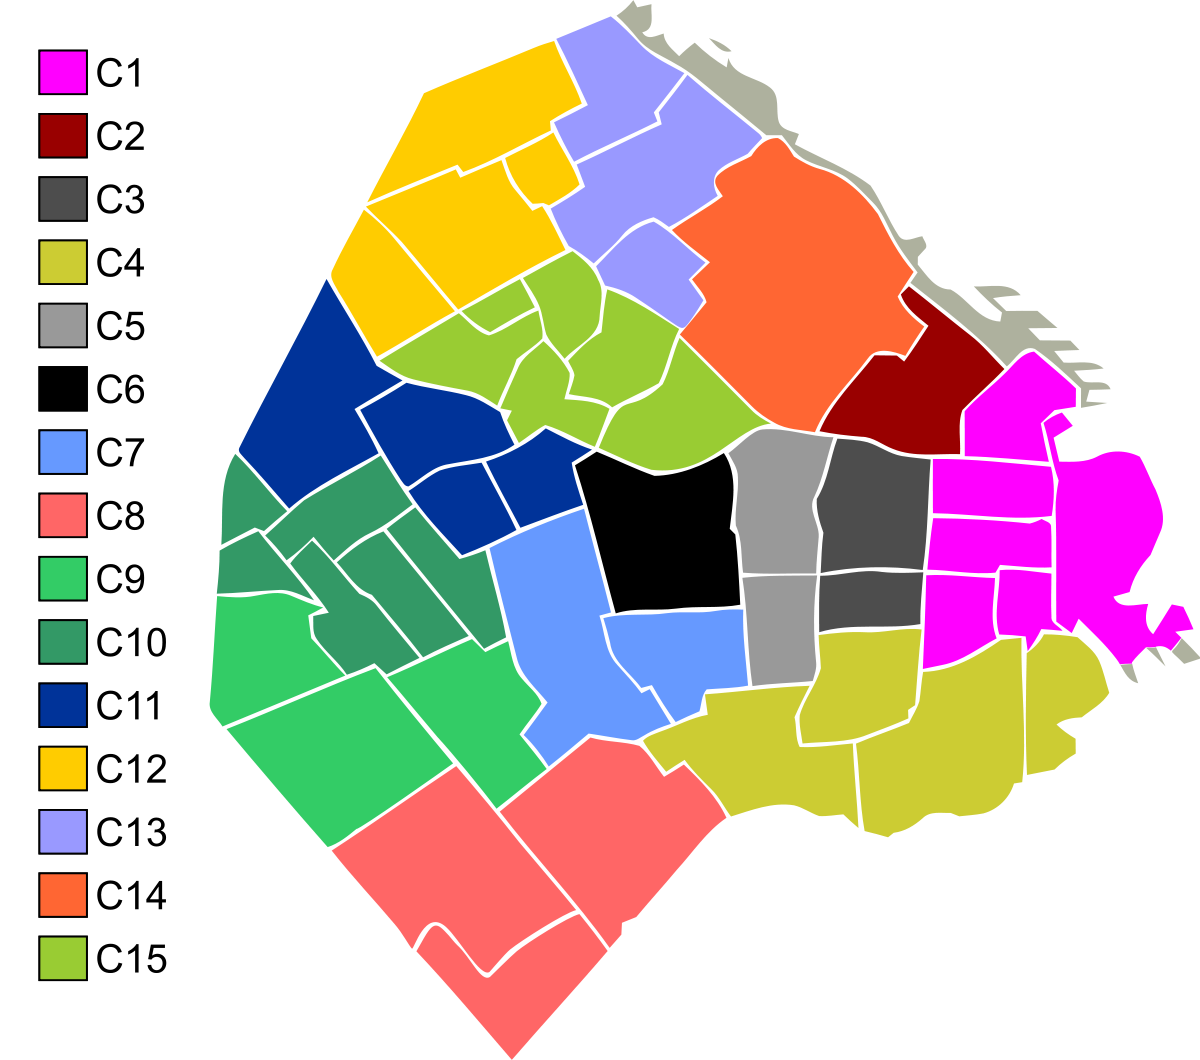
\includegraphics[scale=0.1]{../Informe/Imagenes/Mapa_comunas.jpg}    
    % \end{wrapfigure}

\textbf{Principales hitos:} 
    \begin{itemize}
        \justifying{
        %\item Es de gran importancia desarrollar  políticas públicas que abarquen las necesidades y requerimientos de los ciudadanos. 
        %\item Mediante datos demográficos y la estadística son de gran ayuda para lograr estos fines. El Instituto Nacional de Estadística y Censos (INDEC) es el organismo público que ejerce la dirección superior de todas las actividades estadísticas oficiales que se realizan en Argentina.
        \item Al estudiar los índices correspondientes a uno de los ejes de mayor importancia para la sociedad, educación, en la Ciudad Autónoma de Buenos Aires, se ha encontrado una gran limitación relacionada con su acceso inequitativo para los diferentes actores de la sociedad. 
        % \item Este hecho tiene consecuencias de índole social y económico para la población. Sin embargo, la principal problemática se da a nivel individual, y radica en el impedimento al acceso educativo para un porcentaje de la sociedad. Esto no ha resultado una novedad para el grupo, pero sí ha dado el pie a la búsqueda de una respuesta teórica a dicha disparidad, en concreto, a descubrir las principales variables que afectan el nivel educativo.
        % \item El análisis realizado en el marco del presente proyecto podría establecer una base de requerimientos que permitan generar políticas públicas efectivas, no solo en el ámbito educativo, sino en el económico, cultural, social y geográfico, entre otros.
        \item Para trabajar esta problemática, se ha recurrido a la \href{https://data.buenosaires.gob.ar/dataset/encuesta-anual-hogares/resource/3a45c563-396d-42de-ba93-8a93729e0723}{Encuesta Anual de Hogares} del Gobierno de la Ciudad de Buenos Aires para el año 2019. 
        \item Esta encuesta contiene información demográfica, social, económica, educativa y de salud de 14319 habitantes de la Ciudad, la cual es una muestra representativa que permite obtener un vistazo de la población de la Ciudad.
        } 
    \end{itemize}

   \begin{figure}
        % \centering
        
\includegraphics[scale=0.3]{../Informe/Imagenes/GobCiuBsAs.jpg}
    \end{figure}

\end{frame}

    \subsection{Objetivos del proyecto}

\begin{frame}{Objetivos}

    \begin{itemize}
        \justifying%
        \item Descubrir las principales variables intervinientes en el nivel máximo educativo alcanzado por la población de la Ciudad Autónoma de Buenos Aires (CABA).
        \item Generar un modelo de predicción aplicado a nuestra variable target ``Nivel Máximo Educativo’’, esto lo haremos implementando los siguientes modelos de clasificación:
        \begin{itemize}
            \justifying%
            \item \textbf{Árbol de decisión:} que construye un árbol durante el entrenamiento que es el que aplica a la hora de realizar la predicción.
            \item \textbf{Bosque Aleatorio:} que es un conjunto (ensemble) de árboles de decisión combinados con bagging.
        \end{itemize}
    \end{itemize}

\end{frame}

\section{Planificación}

    \subsection*{Estructura de los trabajos}

\begin{frame}{Estructura de los trabajos}

    Este trabajo se ha dividido en 3 partes:
    \begin{enumerate}
        \justifying%
        \item \textbf{Introducción a las variables del problema:} Se realiza un análisis EDA de las variables del dataset para  conocer su performance dentro del dataset y cómo interactúan entre sí. 
        \item \textbf{Modelos analíticos:} En esta sección se entrenan diversos modelos analíticos y algoritmos que sirven para alcanzar los objetivos seteados para el proyecto. Como la variable objetivo es categórica, se realizan modelos de clasificación.
        \item \textbf{Conclusión:} Se extraen conclusiones finales sobre los hallazgos.
        
        Además, se discuten posibles limitaciones y se plantean futuras líneas de análisis, a partir del análisis presente.

    \end{enumerate}

\end{frame}

\section{Introducción a las variables: Análisis exploratorio de los datos}

\begin{frame}{Análisis exploratorio de los datos (EDA)}
\textbf{Introducción a las variables:}

Encontramos 31 variables dentro de dataset, de las cuales 10 son numéricas y 21 son categóricas. A su vez estas se relaciona con:
\begin{itemize} 
    \item Ingresos
    \item Sector educativo
    \item Factores geográficos
    \item Salud
    \item Descripción del grupo familiar
\end{itemize}
 \vspace{4pt}
 \textbf{Identificación del Target:} En primer lugar transformamos la variable Target (nivel máximo educativo) para reducir su dimensionalidad. Quedando cuatro valores dentro de la variables:  \textbf{Inicial}, \textbf{Prim. Completo}, \textbf{Sec. Completo} y \textbf{Superior}
\end{frame}
 
%     Una ves cargado el dataset con el que vamos a trabajar, miramos sus variable, el tipo que son y si tienen nulls:
%     \begin{table}[H]\begin{center}
%     \begin{tabular}{clll}
%     \multicolumn{4}{l}{RangeIndex: 14319 entries, 0 to 14318} \\
%     \multicolumn{4}{l}{Data columns (total 31 columns):}  \\
%     \#  & Column                     & Non-Null Count & Dtype \\ \hline
%     0  & id                          & 14319 non-null & int64 \\
%     1  & nhogar                      & 14319 non-null & int64 \\
%     2  & miembro                     & 14319 non-null & int64 \\
%     3  & comuna                      & 14319 non-null & int64 \\
%     4  & dominio                     & 14319 non-null & object \\
%     5  & edad                        & 14319 non-null & int64 \\
%     6  & sexo                        & 14319 non-null & object \\
%     7  & parentesco\_jefe             & 14319 non-null & object \\
%     8  & situación\_conyugal          & 14318 non-null & object \\
%     9  & num\_miembro\_padre           & 14319 non-null & object \\
%     10 & num\_miembro\_madre           & 14319 non-null & object \\
%     11 & estado\_ocupacional          & 14319 non-null & object \\
%     12 & cat\_ocupacional             & 14319 non-null & object \\
%     13 & calidad\_ingresos\_lab        & 14319 non-null & object \\
%     14 & ingreso\_total\_lab           & 14319 non-null & int64  \\
%     15 & calidad\_ingresos\_no\_lab     & 14319 non-null & object \\
%     16 & ingreso\_total\_no\_lab        & 14319 non-null & int64  \\
%     17 & calidad\_ingresos\_totales    & 14319 non-null & object \\
%     18 & ingresos\_totales            & 14319 non-null & int64  \\
%     19 & calidad\_ingresos\_familiares & 14319 non-null & object \\
%     20 & ingresos\_familiares         & 14319 non-null & int64  \\
%     21 & ingreso\_per\_capita\_familiar & 14319 non-null & int64  \\
%     22 & estado\_educativo            & 14319 non-null & object \\
%     23 & sector\_educativo            & 14316 non-null & object \\
%     24 & nivel\_actual                & 14319 non-null & object \\
%     25 & nivel\_max\_educativo         & 13265 non-null & object \\
%     26 & años\_escolaridad            & 14257 non-null & object \\
%     27 & lugar\_nacimiento            & 14318 non-null & object \\
%     28 & afiliacion\_salud            & 14315 non-null & object \\
%     29 & hijos\_nacidos\_vivos         & 6535 non-null  & object \\
%     30 & cantidad\_hijos\_nac\_vivos    & 14319 non-null & object \\
%     \multicolumn{4}{l}{dtypes: int64(10), object(21)}  \\
%     \multicolumn{4}{l}{memory usage: 3.4+ MB} \\
%     \end{tabular}\end{center}
%     \end{table}
       
%     Ahora, en base a los datos arrojados por la tabla de arriba, generamos diversas transformaciones de variables, así como la creación de la variable ``Target'', pues es la que usaremos para todo el análisis:
%     \begin{itemize}
%         \item Creamos la variable ``Target'' y le asignamos la variable ``nivel\_max\_educativo''.
%         \item En la variable ``Target'', reducimos su dimensionalidad intercambiando los valores:
%             \begin{itemize}
%                 \item ``Secundario/medio común'' y ``EGB (1° a 9° año)'' por ``sec\_completo'',
%                 \item ``Primario especial'' y ``Primario común'' por ``prim\_completo'',
%                 \item ``Sala de 5'' por ``incial'',
%                 \item ``Otras escuelas especiales" por ``superior'',
%                 \item y por último a ``No corresponde'' por nulos.
%             \end{itemize}
%         \item Remplazamos los valores de ``años\_escolaridad'' para que todos sean numéricos.
%         \item En la variable ``cantidad\_hijos\_nac\_vivos'' cambiamos el valor ``no corresponde'' como nulo, para luego cambiar el tipo de variable a entero.
%         \item Las variables ``comuna'', ``id'', ``nhogar'' y ``miembro'' son de tipo numérico, pero deberían ser categóricas, por lo tanto transformamos su tipo a string.
%         \item Por último renombramos algunas variables para que sean más cortas:
%             \begin{itemize}
%                 \item ``dominio\_Villas\_de\_emergencia'' por ``dominio\_villas'',
%                 \item ``ingreso\_per\_capita\_familiar" por ``ing\_per\_cap\_familiar'',
%                 \item ``cantidad\_hijos\_nac\_vivos'' por ``cant\_hijos\_nac\_vivos''.
%             \end{itemize}
%     \end{itemize}
 
%     A continuación detallamos un diccionario de las variables:
%     \begin{itemize}
%         \item \textbf{``id''}                            : Clave que identifica la vivienda,
%         \item \textbf{``nhogar''}                        : La variable id + nhogar = clave que identifica a cad hogar",
%         \item \textbf{``miembro''}                       : Variables id + nhogar + miembro = clave que identifica  cada persona",
%         \item \textbf{``comuna''}                        : Comuna donde reside la persona encuestada,
%         \item \textbf{``edad''}                          : Edad de la persona encuestada,
%         \item \textbf{``sexo''}                          : Sexo de la persona encuestada,
%         \item \textbf{``parentesco\_jefe''}              : Parentesco entre la persona encuestada y el jefe de hogar,
%         \item \textbf{``situacion\_conyugal''}           : Situación conyugal de la persona encuestada,
%         \item \textbf{``num\_miembro\_padre''}           : Número de miembro que corresponde al padre,
%         \item \textbf{``num\_miembro\_madre''}           : Número de miembro que corresponde a la madre,
%         \item \textbf{``estado\_ocupacional''}           : Situación ocupacional de la persona encuestada,
%         \item \textbf{``cat\_ocupacional''}              : Categoría ocupacional de la persona encuestada,
%         \item \textbf{``calidad\_ingresos\_lab''}        : Calidad de la declaración de ingresos laborales totales,
%         \item \textbf{``ingreso\_total\_lab''}           : Ingreso total laboral percibido el mes anterior,
%         \item \textbf{``calidad\_ingresos\_no\_lab''}    : Calidad de la declaración de ingresos no laborable totales",
%         \item \textbf{``ingreso\_total\_no\_lab''}       : Ingreso total no laboral percibido el mes anterior,
%         \item \textbf{``calidad\_ingresos\_totales''}    : Calidad de ingresos totales individuales,
%         \item \textbf{``ingresos\_totales''}             : Ingreso total individual percibido el mes anterior,
%         \item \textbf{``calidad\_ingresos\_familiares''} : Calidad de ingresos totales familiares,
%         \item \textbf{``ingresos\_familiares''}          : Ingresos totales familiares percibido el mes anterior,
%         \item \textbf{``ing\_per\_cap\_familiar''}       : Ingreso familiar per capita percibido el mes anterior,
%         \item \textbf{``estado\_educativo''}             : Asistencia (pasada o presente) o no a algún establecimiento educativo",
%         \item \textbf{``sector\_educativo''}             : Sector al que pertenece el establecimiento educativo a que asiste",
%         \item \textbf{``nivel\_actual''}                 : Nivel cursado al momento de la encuesta,
%         \item \textbf{``nivel\_max\_educativo''}         : Máximo nivel educativo que se cursó,
%         \item \textbf{``años\_escolaridad''}             : Años de escolaridad alcanzados,
%         \item \textbf{``lugar\_nacimiento''}             : Lugar de nacimiento de la persona encuestada,
%         \item \textbf{``afiliacion\_salud''}             : Afiliación de salud de la persona encuestada,
%         \item \textbf{``hijos\_nacidos\_vivos''}         : Tiene o tuvo hijos nacidos vivos,
%         \item \textbf{``cant\_hijos\_nac\_vivos''}       : Cantidad de hijos nacidos vivos,
%         \item \textbf{``dominio''}                       : ¿La vivienda se ubica en una villa de emergencia?,
%         \item \textbf{``Target''}                        : Nivel máximo educativo.
%     \end{itemize}
 
%     \newpage

%     Y comenzamos el análisis EDA del mismo, primero analizando los nulos:

%     \begin{center}
%         \includegraphics[scale=0.25]{Imagenes/NullsDS.png}
%     \end{center}
 
%     Así, detectamos que nuestra variable target tiene 1054 valores nulos. Es importante tener este dato presente cuando queramos correr un algoritmo de clasificación.

\subsection{Análisis univariado}

    \subsubsection{Género y edad}

\begin{frame}{Análisis univariado}

    Comenzamos con un pantallazo general sobre las primeras cualidades de los datos, como muestra representativa para la EPH, sobre quiénes son los ciudadanos representados en el dataset.

    \begin{center}
        \includegraphics[scale=0.315]{../Informe/Imagenes/AUGenero.png}
    \end{center}

    En la variable género los datos parecen equilibrados en las categorías. Para el caso de la variable ``edad'', la distribución se asemeja a la de una normal.

\end{frame}
              
%     \subsubsection{Comuna}

% \begin{frame}{Análisis univariado}

%     Seguimos observando la variable ``comuna'':
%     \begin{center}
%         \includegraphics[scale=0.236]{../Informe/Imagenes/AUComuna.png}    
%     \end{center}
%     Observando ambos gráficos vemos que las comunas 1,4,7 y 8 tienen mayor cantidad de casos.
    
% \end{frame}
           
%     \subsubsection{Ingreso familiar per cápita}

% \begin{frame}{Análisis univariado}

%     \begin{center}
%         \includegraphics[scale=0.236]{../Informe/Imagenes/AUIngFam.png}
%     \end{center}

% \end{frame}

%             Ahora probamos con observar los ingresos familiares. Creemos que puede ser un indicador interesante del nivel educativo.
           
%             Para esto, armamos una función para graficar y jugar con el nivel del filtrado de la variable y obtener un histograma que permita apreciar mejor la distribución de la variable sin tantos outliers:
           
%             % Y como hay muchos outliers que impiden ver la distribución correctamente, los quitamos de los gráficos:
           
%             % \includegraphics[scale=0.4]{Graf5.png}
 
%             Y luego de remover los outliers la distribución de los ingresos familiares sigue estando \textbf{sesgada}.

%             \subsubsection{Años de escolaridad}
           
%             Analizamos mediante un gráfico de barras los años de escolaridad alcanzados por los encuestados:
           
%             \begin{center}
%                 \includegraphics[scale=0.6]{Imagenes/AUAnosEsc.png}
%             \end{center}
           
%             A simple vista se observan tres "picos": en el valor mínimo, alrededor del 7.5 y alrededor del 12.5. Podemos inferir que estos tres casos corresponden a no tener estudios, solo haber transcurrido el primario y haber transcurrido hasta la educación secundaria, respectivamente.
           
    \subsubsection{Máximo nivel educativo (Target)}
    
\begin{frame}{Análisis univariado}
    Cuando observamos el \textbf{nivel máximo educativo} encontramos que el más alcanzado es el secundario completo, seguido por el primario. Contrario de lo que habíamos intuido anteriormente, el nivel superior quedó en tercer lugar. Adicionalmente, el nivel secundario y primario explican casi el 77\% de los datos.
  
    \begin{center}
        \includegraphics[scale=0.225]{../Informe/Imagenes/AUTarget.png}    
    \end{center}

\end{frame}
    
    \subsection{Análisis bivariado}

\begin{frame}{Análisis bivariado}
    \vspace{-20pt}
    \textbf{Variable numéricas:}
    \vspace{4pt}

    Realizamos un mapa de calor para ver la interacción entre las variables numéricas.

    \begin{minipage}{0.46\textwidth}
        \vspace{10pt}
        \includegraphics[scale=0.22]{../Informe/Imagenes/ABSpearman.png}
    \end{minipage}
    \begin{minipage}{0.46\textwidth}
        \vspace{4pt}
        \begin{itemize}
            \justifying%
            \item No se observan fuertes correlaciones.
            \item ``años\_escolaridad'' correlaciona moderadamente bien con variables relacionadas al ingreso.
            \item La principal correlación positiva es ``años\_escolaridad'' con ingreso familiar per cápita (``ing\_per\_cap\_familiar'').
        \end{itemize}
    \end{minipage}

\end{frame}
 
%         Ahora, utilizando el método para solo graficar en base a un threshold vemos que los años de escolaridad alcanzados por los entrevistados tienen algo relación $(66\%$) con la variable ``ingresos\_totales''
%         % Estaría bien solo utilizar el gráfico de la derecha.

%         \begin{center}
%             \includegraphics[scale=0.4]{Imagenes/ABThreshold.png}
%         \end{center}
 
% \begin{frame}{Análisis bivariado}

    % Corremos una tabla de correlación y filtramos las de valores más altos:
 
    % \begin{table}[H]
    %     \centering
    %     \begin{tabular}{|l|l|l|l|}
    %     \hline
    %         ~ & Variable 1 & Variable 2 & Correlación \\ \hline
    %         2 & ingreso\_total\_lab & ingresos\_totales & 0.80 \\ \hline
    %         6 & ingresos\_familiares & ing\_per\_cap\_familiar & 0.76 \\ \hline
    %         4 & ingresos\_totales & ing\_per\_cap\_familiar & 0.62 \\ \hline
    %         5 & ingresos\_totales & años\_escolaridad & 0.60 \\ \hline
    %         1 & edad & ingreso\_total\_no\_lab & 0.57 \\ \hline
    %         7 & años\_escolaridad & Target & 0.57 \\ \hline
    %         3 & ingreso\_total\_lab & años\_escolaridad & 0.54 \\ \hline
    %     \end{tabular}
    % \end{table}

%     \begin{itemize}
%         \justifying
%         \item Como es esperable, hay alta correlación entre las variables relacionadas al ingreso.
%         \item A su vez, encontramos una alta correlación (66\%) entre los ingresos y los años de escolaridad.
%         \item Y también observamos una relación positiva entre la edad y los ingresos totales.
%     \end{itemize}

% \end{frame}
 
    \subsubsection{Comparación entre variables numéricas}

\begin{frame}{Análisis bivariado}

    Observamos la relación entre los ingresos totales de cada hogar y los ingresos familiares por edad:
    \begin{center}
        \includegraphics[scale=0.15]{../Informe/Imagenes/ABCompVarNum.png}
    \end{center}
    Se puede ver que desde los 30 años en adelante el ingreso total de la persona se corresponde con el ingreso familiar. Por ende suele haber un único ingreso fuerte por grupo familiar.

\end{frame}
 
    \subsubsection{Comparación de variables categóricas con numéricas}

\begin{frame}{Análisis bivariado}

    \textbf{Variable numéricas y categóricas}
    \vspace{6pt}

    Adicionalmente, comparamos algunas variables con nuestro target, comenzando con los ingresos totales.

%     \begin{center}
%         \includegraphics[scale=0.157]{../Informe/Imagenes/ABCatVsNum1.png}
%     \end{center}

% \end{frame}

% \begin{frame}{Análisis bivariado}
%     \footnotesize

%     Veamos como se relacionan las categorías de ingresos con el genero de los encuestados:
%     \begin{center}
%         \includegraphics[scale=0.295]{../Informe/Imagenes/ABCatVsNum2.png}
%     \end{center}
%     Y resulta que con las variables de ingreso, no parece haber nada disruptivo. Salvo que los hombres parecieran tener ingresos totales y familiares mayores que las mujeres, pero no pareciera que haya distribuciones desiguales en los años de escolaridad.

% \end{frame}

%             Probemos quitando outliers, a excepción de la cantidad de hijos nacidos vivos (puesto que no arrojará ningún dato nuevo) y de años de escolaridad (que no tiene outliers)
 
%             \begin{center}
%                 \includegraphics[scale=0.425]{Imagenes/ABCatVsNum2.png}
%             \end{center}
 
%             Por parte de las variables de ingreso, no parece haber nada disruptivo. La distribución por ingreso y años de escolaridad pareciera ocurrir pero no en un orden lineal.
 
%             Llama la atención la variable ``sexo'': que por algún motivo, todos los encuestados hombres figuran sin hijos nacidos vivos. Alternativamente, se podría investigar la metodología de la encuesta para ver si hay alguna respuesta. Adicionalmente, los hombres parecieran tener ingresos totales y familiares mayores que las mujeres, pero no pareciera que haya distribuciones desiguales en los años de escolaridad.

    \begin{figure}
        \includegraphics[
                         width=13cm,
                         height=4cm
                         ]{../Informe/Imagenes/ABCatVsNum3Bis.png}
    \end{figure}

\end{frame}


    % Parece que para el nivel inicial la remoción de outliers en otra categoría sigue siendo insuficiente para mostrar la distribución real de la variable. Echemos un vistazo a los valores de esta categoría:
 
%             \begin{center}
%                 \includegraphics[scale=0.3]{Imagenes/ABCatVsNum3Bis.png}
%             \end{center}
 
%             Parece que para el nivel inicial la remoción de outliers en otra categoría sigue siendo insuficiente para mostrar la distribución real de la variable. Echemos un vistazo a los valores de esta categoría:
 
% \begin{frame}{Análisis bivariado}
%     \footnotesize

%     \begin{center}
%         \includegraphics[scale=0.5]{../Informe/Imagenes/ABCatVsNum4.png}
%     \end{center}

%     Lógicamente, la enorme mayoría de los ingresos tienen el valor inicial de 0, puesto que incluye a personas que en ese momento estaban cursando su educación inicial, por lo que tenían entre 2 y 6 años.

% \end{frame}

\begin{frame}{Análisis bivariado}

    Más aún, analizamos como se distribuyen los ingresos familiares con respecto a nuestro target:

    \begin{center}
        \includegraphics[scale=0.21]{../Informe/Imagenes/ABCatVsNum5.png}
    \end{center}

    En definitiva, se observa un desplazamiento de los valores centrales (dentro de la caja) hacia la izquierda a medida que aumenta el nivel educativo.


\end{frame}

    \subsubsection{Variable numéricas con comuna}

\begin{frame}{Análisis bivariado}
    \footnotesize
    
    Por último, analizamos la relación de nuestro target en cada comuna:

    \begin{minipage}{0.55\textwidth}
        \vspace{10pt}
        \includegraphics[scale=0.25]{../Informe/Imagenes/ABCatVsNum6.png}
    \end{minipage}
    \begin{minipage}{0.4\textwidth}
        \begin{itemize}
            \vspace{-10pt}
            \justifying%
            \item En el sur de la ciudad hay mayor cantidad de encuestados con niveles de inicial, primario y secundario completo,
            \item Mientras que el norte (particularmente el barrio de Palermo) tiene mayor cantidad de personas con estudios superiores,
            \item En menor medida también las comunas del este (comúnmente llamado el ``centro de la ciudad'') destacan por la cantidad de encuestados con nivel superior.
        \end{itemize}
    \end{minipage}

\end{frame}    

% \begin{frame}{Análisis bivariado}
    
%     Lo que podemos observar en los últimos dos gráficos es una clara división geográfica del nivel educativo:

%     \begin{minipage}{0.44\textwidth}
%         \includegraphics[scale=0.23]{../Informe/Imagenes/ABCatVsNum7.png}
%     \end{minipage}
%     \begin{minipage}{0.51\textwidth}
%         \begin{itemize}
%             \justifying
%             \item Las comunas del norte son las que tienen mayor nivel educativo.
%             \item Las comunas del centro tienen niveles medios.
%             \item Las comunas del sur (con las comuna 6 en el centro de la ciudad como outlier) y la comuna 1 en el este son las que tienen niveles más bajos.
%         \end{itemize}
%     \end{minipage}

% \end{frame}

    \subsection{Análisis multivariado}

\begin{frame}{Análisis multivariado}
    \footnotesize

    Probamos de cruzar años de escolaridad, nivel máximo educativo y los ingresos totales.
    \vspace{10pt}

    \begin{minipage}{0.6\textwidth}
        \includegraphics[scale=0.3]{../Informe/Imagenes/AMIngVsAnosEsc.png}
    \end{minipage}
\begin{minipage}{0.39\textwidth}


    Al visualizar el gráfico podemos observar que:

    \begin{itemize}
        \footnotesize
        \justifying%
        \item Hasta los 6 años, como era esperable, todos los casos llegan al nivel inicial.
        \item Vemos dos años en que aparece el primario completo: 7 y 12 años. Estimamos que se debe a la división entre los que comenzaron su educación en la primaria y los que comenzaron en el nivel inicial.
        \item A partir de los 12 años vemos un aumento consistente de los ingresos totales.
    \end{itemize}
\end{minipage}
\end{frame} 

\begin{frame}{Análisis multivariado}

    \footnotesize

    Añadimos una variable más: dominio =``villas\_de\_emergencia'':
    \vspace{-5pt}

    \begin{figure}[H]
        \includegraphics[width=\textwidth,
                         height=7cm]{../Informe/Imagenes/AMIngVSTargetBis.png}
    \end{figure}
    \vspace{-18pt}
    
    Podemos ver que los casos que no provienen de villas de emergencia  obtienen en promedio ingresos más altos en todos los niveles educativos. El alcanzar estudios superiores no parece homogeneizar ambos conjuntos. 

\end{frame}

%Esto se puede sacar/prescindir 
\begin{frame}{Análisis multivariado}

    Luego, observamos los ingresos familiares según el máximo nivel educativo alcanzado:

    \begin{minipage}{0.55\textwidth}
        % \vspace{5pt}
        \begin{figure} 
        \includegraphics[scale=0.26]{../Informe/Imagenes/AMIngVsComuna.png}
        \caption{Figure X}
        \end{figure}
    \end{minipage}
    \begin{minipage}{0.38\textwidth}
        \begin{itemize}
            \justifying%
            \item a medida que avanza el nivel educativo máximo se atenúan levemente las diferencias de ingresos familiares entre comunas,
            \item queda pendiente cruzar estos datos con la edad, para saber si el hecho de incluir a menores de edad está sesgando los valores para nivel inicial, primario y secundario.
        \end{itemize}
    \end{minipage}

\end{frame}

\section{Modelos analíticos}

\begin{frame}{Modelos analíticos}

    Transformamos variables para poder trabajar con los algoritmos:
    \begin{itemize}
        \item recategorizando la variables ``Target'' en variables numéricas, es decir, a cada nivel educativo le asignamos un valor numérico del 1 al 4:
        \begin{itemize}
            \item \textbf{inicial=} 1,
            \item \textbf{prim\_completo=} 2,
            \item \textbf{sec\_completo=} 3,
            \item \textbf{superior=} 4,
        \end{itemize}
        \item reagrupamos la variable ``comuna'' por regiones para reducir la dimensionalidad (en norte, centro, sur y oeste),
        \item eliminamos algunas variables que no resultan relevantes, 
        \item renombramos algunas variables para que sean más cortas.
    \end{itemize}
    
\end{frame}

%     Como resultado nos quedan las siguientes variables:
    
%     \begin{table}[H]
%         \centering
%         \begin{tabular}{clll}
%             \multicolumn{4}{l}{RangeIndex: 14319 entries, 0 to 14318} \\
%             \multicolumn{4}{l}{Data columns (total 33 columns):} \\
%             \#  & features & types & non\_null\_counts \\ \hline 
%             0   & id & object & 14319 \\ 
%             1   & nhogar & object & 14319 \\ 
%             2   & miembro & object & 14319 \\ 
%             3   & comuna & object & 14319 \\ 
%             4   & dominio & object & 14319 \\ 
%             5   & edad & int64 & 14319 \\ 
%             6   & sexo & object & 14319 \\ 
%             7   & parentesco\_jefe & object & 14319 \\ 
%             8   & situacion\_conyugal & object & 14318 \\ 
%             9   & num\_miembro\_padre & object & 14319 \\ 
%             10  & num\_miembro\_madre & object & 14319 \\ 
%             11  & estado\_ocupacional & object & 14319 \\ 
%             12  & cat\_ocupacional & object & 14319 \\ 
%             13  & calidad\_ingresos\_lab & object & 14319 \\ 
%             14  & ingreso\_total\_lab & int64 & 14319 \\ 
%             15  & calidad\_ingresos\_no\_lab & object & 14319 \\ 
%             16  & ingreso\_total\_no\_lab & int64 & 14319 \\ 
%             17  & calidad\_ingresos\_totales & object & 14319 \\ 
%             18  & ingresos\_totales & int64 & 14319 \\ 
%             19  & calidad\_ingresos\_familiares & object & 14319 \\ 
%             20  & ingresos\_familiares & int64 & 14319 \\ 
%             21  & ing\_per\_cap\_familiar & int64 & 14319 \\ 
%             22  & estado\_educativo & object & 14319 \\ 
%             23  & sector\_educativo & object & 14316 \\ 
%             24  & nivel\_actual & object & 14319 \\ 
%             25  & nivel\_max\_educativo & object & 13265 \\ 
%             26  & años\_escolaridad & float64 & 14257 \\ 
%             27  & lugar\_nacimiento & object & 14318 \\ 
%             28  & afiliacion\_salud & object & 14315 \\ 
%             29  & hijos\_nacidos\_vivos & object & 6535 \\ 
%             30  & cant\_hijos\_nac\_vivos & int64 & 14319 \\ 
%             31  & Target & Int64 & 13223 \\ 
%             32  & region & object & 14319 \\
%             \multicolumn{4}{l}{dtypes: Int64(1), float64(1), int64(7), object(24)} \\
%             \multicolumn{4}{l}{memory usage: 3.6+ MB } \\
%         \end{tabular}
%     \end{table}

    \subsection{Tratados de nulos}

\begin{frame}{Modelos analíticos}

    \begin{Large}
        \textbf{Tratados de nulos}
    \end{Large}
    \vspace{4pt}

    Encontramos valores nulos en estas variables, por lo que para trabajar con el modelado los remplazamos con las siguientes métricas:

    \begin{table}[H]
        \begin{tabular}{lrl}
            \toprule
            \textbf{Variable}                & \textbf{Nulos} & \textbf{Acción} \\ \midrule
            situacion\_conyugal     & 1     & Reemplazamos con la moda\\ 
            lugar\_nacimiento       & 1     & Reemplazamos con la moda\\ 
            sector\_educativo       & 3     & Reemplazamos con la moda\\ 
            afiliacion\_salud       & 4     & Reemplazamos con la moda\\ 
            años\_escolaridad       & 62    & Reemplazamos con la \\
                                    &       & mediana por comuna y sexo\\ 
            nivel\_max\_educativo   & 1054  & Eliminamos la variable\\ 
            Target                  & 1096  & Eliminamos sus nulos y transformamos\\
                                    &       & su tipo a entero\\ 
            hijos\_nacidos\_vivos   & 7784  & Reemplazamos con la moda\\ 
            \bottomrule
        \end{tabular}
    \end{table}
    
\end{frame}

    \subsection{Target}

        \subsubsection{Borrado de variables}

% \begin{frame}{Modelos analíticos}
%     \scriptsize
%         Hay muchas variables que consideramos que no es necesario sumarlas al algoritmo de clasificación dado que brindan información repetida o que no suma para la clasificación. A continuación se comparten las categoría que se descartarán para correr el algoritmo: 
%         \begin{itemize}
%             \item \textbf{id:} no suma información para la clasificación,
%             \item \textbf{nhogar:} no suma información para la clasificación,
%             \item \textbf{parentesco\_jefe:} no suma información para la clasificación,
%             \item \textbf{miembro:} no suma información para la clasificación,
%             \item \textbf{num\_miembro\_padre:} no suma información para la clasificación,
%             \item \textbf{num\_miembro\_madre:} no suma información para la clasificación,
%             \item \textbf{cat\_ocupacional:} brinda la misma información que estado\_ocupacional,
%             \item \textbf{calidad\_ingresos\_lab:} brinda la misma información que ingreso\_total\_lab,
%             \item \textbf{calidad\_ingresos\_no\_lab:} brinda la misma información que ingreso\_total\_no\_lab,
%             \item \textbf{calidad\_ingresos\_totales:} brinda la misma información que ingresos\_totales,
%             \item \textbf{calidad\_ingresos\_familiares:} brinda la misma información que ingreso\_familiares,
%             \item \textbf{estado\_educativo:} no aporta información para la clasificación,
%             \item \textbf{nivel\_actual:} no aporta información para la clasificación,
%             \item \textbf{hijos\_nacidos\_vivos:} brinda la misma información que cant\_hijos\_nac\_vivos,
%             \item \textbf{comuna:} variable ya abordada en la variable 'región'.
%         \end{itemize}

%     Por último eliminamos algunas variables que no tienen importancia, y tenemos nuestro dataset listo para el procesamiento:

%     \begin{table}[H]
%         \centering
%         \begin{tabular}{clll}
%             \multicolumn{4}{l}{RangeIndex: 14319 entries, 0 to 14318} \\
%             \# & features & types & non\_null\_counts \\ \hline
%             0 & dominio & object & 13223 \\ 
%             1 & edad & int64 & 13223 \\ 
%             2 & sexo & object & 13223 \\ 
%             3 & situacion\_conyugal & object & 13223 \\ 
%             4 & estado\_ocupacional & object & 13223 \\ 
%             5 & ingreso\_total\_lab & int64 & 13223 \\ 
%             6 & ingreso\_total\_no\_lab & int64 & 13223 \\ 
%             7 & ingresos\_totales & int64 & 13223 \\ 
%             8 & ingresos\_familiares & int64 & 13223 \\ 
%             9 & ing\_per\_cap\_familiar & int64 & 13223 \\ 
%             10 & sector\_educativo & object & 13223 \\ 
%             11 & años\_escolaridad & float64 & 13223 \\ 
%             12 & lugar\_nacimiento & object & 13223 \\ 
%             13 & afiliacion\_salud & object & 13223 \\ 
%             14 & cant\_hijos\_nac\_vivos & int64 & 13223 \\ 
%             15 & Target & int32 & 13223 \\ 
%             16 & region & object & 13223 \\ 
%             \multicolumn{4}{l}{dtypes: Int64(1), float64(1), int64(7), object(8)} \\
%             \multicolumn{4}{l}{memory usage: 2.0+ MB} 
%         \end{tabular}
%     \end{table}

% \end{frame}

        \subsection{Procesamiento}

\begin{frame}{Modelos analíticos}

    \begin{Large}
        \textbf{Procesamiento}
    \end{Large}
    \vspace{6pt}

    Para preparar los datos para el modelado generamos una función que:
    
    \vspace{6pt}
    \begin{itemize}
        \justifying%
        \item  Divide el dataframe en X\_train, y\_train, X\_test e y\_test, haciendo la división entre test y el train en un 30\% y un 70\% respectivamente, con una semilla especifica.
        
        \vspace{6pt}
        \item  Procesa el X\_train y el X\_test con un pipeline generado previamente, el cual convierte las variable numéricas con el minmaxscaler y las categóricas con one hot encoding.
    \end{itemize}



\end{frame}

    \subsection{Árbol de decisión}

        

\begin{frame}{Modelos analíticos}

    \begin{Large}
        \textbf{Árbol de decisión}
    \end{Large}

     \textbf{1. Primer modelo:}

    Como punto de partida usamos un árbol de clasificación con parámetros:
    \begin{itemize}
        \item random\_state = 50,
        \item max\_depth=8,
        \item criterion='gini',
    \end{itemize}

    El Accuracy score para el test es de: 0.940 y las métricas

    \begin{table}[H]
        \scriptsize
        \centering
        \begin{tabular}{rcccc}
            \toprule
             & precision & recall & f1-score & support \\ \midrule
            Inicial    & 1.00& 1.00 & 1.0 & 446 \\ 
            Primario   & 0.93 & 0.99 & 0.95 & 978 \\ 
            Secundario & 0.95 & 0.96 & 0.95 & 1771 \\ 
            Superior   & 0.90 & 0.82 & 0.86 & 772 \\ 
            & & & & \\
            accuracy & & & 0.94 & 3967 \\ 
            macro avg & 0.94 & 0.94 & 0.94 & 3967 \\ 
            weighted avg & 0.94 & 0.94 & 0.94 & 3967 \\ 
            \bottomrule
        \end{tabular}
    \end{table}
\end{frame}

\begin{frame}{Modelos analíticos}
    \begin{Large}
        \textbf{Resultados}
    \end{Large}
     \begin{itemize}
          \item \textbf{Bias o sesgo:} 96.89\% que nos indica que tengo poco error, lo que indica que tenemos un sesgo bajo,
         \item \textbf{Variance=Test\_Score $-$ Bias=} 2.89\%, lo que nos indica que la varianza también es baja.
     \end{itemize}

    \vspace{6pt}
    
    Entonces, el modelo tiene una \textbf{buena relación} de sesgo y varianza.

\vspace{10pt}
    
Sin embargo, tenemos que la variable ``años\_escolaridad'' tiene una importancia del 84\%, por mucho superior al resto de variables.

    % Tendríamos que agregar algo relacionado a la diferencia que tenemos con los resultado del EDA.
\vspace{10pt}

    Por lo tanto, desarrollamos un nuevo modelo sin esta variable. 

\end{frame}

        \subsubsection{Segundo modelo}

\begin{frame}{Modelos analíticos}
    \textbf{2. Segundo modelo:}
    
    Esta vez al correr el modelo, utilizaremos el ``DecisionTreeClassifier'' solo con los parámetros:
    \begin{itemize}
        \item random\_state = 50,
        \item cirterion='entropy'.
    \end{itemize}
    Que nos da como resultado:  

    \begin{table}[!ht]
        \scriptsize
        \centering
        \begin{tabular}{rcccc}
            \toprule
             & precision & recall & f1-score & suppo \\ \midrule
            Inicial    & 0.83 & 0.79 & 0.81 & 446 \\
            Primario   & 0.45 & 0.26 & 0.33 & 978 \\
            Secundario & 0.56 & 0.66 & 0.60 & 1771 \\
            Superior   & 0.39 & 0.45 & 0.42 & 772 \\
            & & & & \\
            accuracy & & & 0.53 & 3967 \\
            macro avg & 0.56 & 0.59 & 0.54 & 3967 \\
            weighted avg & 0.53 & 0.53 & 0.52 & 3967 \\
            \bottomrule
        \end{tabular}
    \end{table}

\end{frame}

\begin{frame}{Modelos analíticos}

    \begin{Large}
        \textbf{Resultados}
    \end{Large}
    \vspace{6pt}
    \begin{itemize}
        \item \textbf{Bias o sesgo:} 99.78\% que nos indica que tengo poco error, es decir, un sesgo bajo,
        \item \textbf{Variance=Test\_Score $-$ Bias=} 46.39\%, lo que nos indica un nivel de varianza bastante alto,
    \end{itemize}

    Lo que nos da como resultado, que este modelo esta haciendo 
    
    \textbf{OVERFITTING}.

\vspace{10pt}

    Por lo que se observa, el árbol performa bastante peor sin esta variable, aumentando especialmente la varianza. Por lo tanto optamos probar mejorar nuestro modelo con un grid search.

\end{frame}

\subsubsection{Gridsearch con CV}

\begin{frame}{Modelos analíticos}
    \begin{Large}
        \textbf{Gridsearch con CV}
    \end{Large}
    \vspace{6pt}
    
    En la grilla de parámetros para el Gridsearch elegimos los siguientes:
    \begin{itemize}
        \item max\_depth: $range(5,11)$,
        \item max\_features: $range(1,14)$,
        \item criterion: [`gini', `entropy',`log\_loss'];
    \end{itemize}

\vspace{10pt}
    como estimador el ``DecisionTreeClassifier'' con el random\_state=50, con el cross-validation =10,  usando todos los procesadores.

\vspace{10pt}

    Y nos da como resultado, que el mejor árbol de decisión posible obtiene 0.642. Y para eso el árbol debe tener una profundidad de  6, utilizar  10  variables y usar el método ``gini''.

\end{frame}

\begin{frame}{Modelos analíticos}
    
    \begin{Large}
        \textbf{Gridsearch con CV}
    \end{Large}

\vspace{10pt}

    Entonces, entrenamos el modelo bajo estos mismos parámetros y obtenemos el siguiente reporte de clasificación:

    \begin{table}[H]
        \scriptsize
        \centering
        \begin{tabular}{rcccc}
            \toprule
             & precision & recall & f1-score & suppo \\ \midrule
            Inicial    & 0.99 & 0.74 & 0.85 & 446 \\
            Primario   & 0.49 & 0.21 & 0.30 & 978 \\
            Secundario & 0.55 & 0.87 & 0.69 & 1771 \\
            Superior   & 0.78 & 0.41 & 0.54 & 772 \\
            accuracy & & & 0.60 & 3967 \\
            macro avg & 0.70 & 0.56 & 0.59 & 3967 \\
            weighted avg & 0.63 & 0.60 & 0.57 & 3967 \\
            \bottomrule
        \end{tabular}
    \end{table}
\end{frame}

\begin{frame}{Modelos analíticos}

    \begin{Large}
        \textbf{Resultados}
    \end{Large}
    
\vspace{6pt}    
    \begin{itemize}
        \item \textbf{Bias o sesgo:} 65.27\% que nos indica que tengo bastantes errores $\Rightarrow$ high bias,
        \item \textbf{Variance=Test\_Score $-$ Bias:} 5.14\%  $\Rightarrow$ low variance.
    \end{itemize}
    
\vspace{6pt} 

    Por lo tanto, el modelo esta haciendo \textbf{UNDERFITTING}
    
\vspace{6pt}    

    Utilizar el grid search nos permitió mejorar bastante el modelo que había perdido bastante accuracy al retirar los años de escolaridad. 
    
\vspace{6pt}
    
    La métrica que más pudimos mejorar con este método fue la varianza, que pasó de 44.97\% a 5.14\%, pero en contra parte nuestro acuracy bajo de 100\% a 65.27\%.

\end{frame}

    \subsection{Random Forest Classifier}

\begin{frame}{Modelos analíticos}

    
    \begin{Large}
        \textbf{Random Forest Classifier}
    \end{Large}

\vspace{10pt}

    \textbf{3. Tercer modelo:}
    
\vspace{6pt}

    En esta instancia hemos teniendo en cuenta todo el dataset incluido la variable con los años de escolaridad. 
    
\vspace{6pt}

    Como tercer modelo con el Random Forest Classifier, elegimos los siguientes parámetros:
    \begin{itemize}
        \item n\_estimators=200,
        \item max\_depth=15,
        \item random\_state=50,
        \item criterion='gini.
    \end{itemize}

\end{frame}

\begin{frame}{Modelos analíticos}

    \begin{Large}
        \textbf{Random Forest Classifier}
    \end{Large}
\vspace{6pt}
    
        Que nos da los siguientes resultados en cuanto a las métricas:
        \begin{table}[H]
            \scriptsize
            \centering
            \begin{tabular}{rcccc}
                \toprule
                 & precision & recall & f1-score & suppo \\ \midrule
                Inicial    & 1.00 & 0.96 & 0.98 & 446 \\
                Primario   & 0.86 & 0.95 & 0.90 & 978 \\
                Secundario & 0.91 & 0.93 & 0.9 & 1771 \\
                Superior   & 0.92 & 0.76 & 0.83 & 772 \\
                & & & & \\
                accuracy & & & 0.91 & 3967 \\
                macro avg & 0.92 & 0.90 & 0.91 & 3967 \\
                weighted avg & 0.91 & 0.91 & 0.90 & 3967 \\
                \bottomrule
            \end{tabular}
        \end{table}

    El random forest performa bastante bien, es decir, mucho mejor que los modelos anteriores.
\end{frame}

\begin{frame}{Modelos analíticos}

    \begin{Large}
        \textbf{Resultados}
    \end{Large}
    \vspace{6pt}    
    
    \begin{itemize}
    \item \textbf{Bias o sesgo:} 97.80\% que nos indica que tengo bastantes errores, es decir tenemos un sesgo alto,
    \item \textbf{Variance=Test\_Score $-$ Bias:} 7.20\%, que nos indica que la varianza es baja.
    \end{itemize}

    Obtuvimos un buen modelo. No obstante, buscamos cuales son las variables más importantes, y encontramos que los años de escolaridad redujo la enorme importancia (a un 43.58\%) que tenía en el random tree. 
    
    \vspace{10pt}
    
    Sin embargo, sigue correspondiendo quitarla del modelo.

\end{frame}

\subsubsection{Cuarto modelo}

\begin{frame}{Modelos analíticos}

    \textbf{4. Cuarto modelo:}
   
\vspace{6pt}

    En este caso elegimos los siguientes parámetros:
    \begin{itemize}
        \item n\_estimators=200,
        \item max\_depth=10,
        \item random\_state=50,
        \item criterion='gini'.
    \end{itemize}

    Dándonos por resultado los siguientes medidas de desempeño:
    \begin{table}[H]
        \scriptsize
        \centering
        \begin{tabular}{rcccc}
            \toprule
             & precision & recall & f1-score & suppo \\ \midrule
            Inicial    & 0.95 & 0.78 & 0.86 & 446 \\
            Primario   & 0.54 & 0.23 & 0.32 & 978 \\
            Secundario & 0.56 & 0.88 & 0.69 & 1771 \\
            Superior   & 0.80 & 0.40 & 0.53 & 772 \\
            & & & & \\
            accuracy & & & 0.62 & 3967 \\
            macro avg & 0.71 & 0.57 & 0.60 & 3967 \\
            weighted avg & 0.65 & 0.62 & 0.59 & 3967 \\
            \bottomrule
        \end{tabular}
    \end{table}

\end{frame}

\begin{frame}{Modelos analíticos}
    \begin{Large}
        \textbf{Resultados}
    \end{Large}

\vspace{6pt}    
    En este caso  obtuvimos los siguientes valores del sesgo y la varianza:
    \begin{itemize}
        \item \textbf{Bias o sesgo:} 89.11\% que nos indica que tengo pocos errores, es decir, que el sesgo es bastante bajo,
        \item \textbf{Variance=Test\_Score $-$ Bias=} 27.4\%, esto indica que tenemos un valor alto en la varianza.
        \end{itemize}

    El modelo empeora su accuracy pero está muy cercano al mejor modelo de Random Tree, mientras que crece mucho la varianza a un 27.4\% (unos 20 puntos). Ahora, al igual que con el el DesicionTree, vamos a probar mejorándolo con grid search.

\end{frame}

    \subsubsection{Gridsearch con CV}

\begin{frame}{Modelos analíticos}

    \begin{Large}
        \textbf{Gridsearch con CV}
    \end{Large}
    \vspace{6pt}

    En la grilla de parámetros para el Gridsearch elegimos los siguientes:
    \begin{itemize}
        \item max\_depth: [5,7,10,15,None],
        \item max\_features: [5,8,10,30,41],
        \item n\_estimators: [200,300,500],
        \item criterion: [`gini',`entropy',`log\_loss'].
    \end{itemize}
    como estimador el ``RandomTreeClassifier'' que utilizamos en el último modelo, con el cross-validation =10 y  usando todos los procesadores.

    Y nos da como resultado, que el mejor random forest posible obtiene 0.668. 

    Y para eso el árbol debe tener una profundidad de 15, utilizar  10  variables, tener  300  estimadores y utilizar el método ``gini''.

\end{frame}

\begin{frame}{Modelos analíticos}    

    \begin{Large}
        \textbf{Gridsearch con CV}
    \end{Large}
    
    \vspace{6pt}
        Entonces, entrenamos el modelo bajo estos mismos parámetros y obtenemos el siguiente reporte de clasificación:

    \begin{table}[!ht]
        \scriptsize
        \centering
        \begin{tabular}{rcccc}
            \toprule
             & precision & recall & f1-score & support \\ \midrule
            Inicial    & 0.95 & 0.79 & 0.86 & 446 \\
            Primario   & 0.56 & 0.23 & 0.33 & 978 \\
            Secundario & 0.56 & 0.89 & 0.69 & 1771 \\
            Superior   & 0.80 & 0.40 & 0.54 & 772 \\
            & & & & \\
            accuracy & & & 0.62 & 3967 \\
            macro avg & 0.72 & 0.58 & 0.60 & 3967 \\
            weighted avg & 0.65 & 0.62 & 0.59 & 3967 \\
            \bottomrule
        \end{tabular}
    \end{table}
\end{frame}

\begin{frame}{Modelos analíticos}
    \begin{Large}
        \textbf{Resultados}
    \end{Large}
    
    \vspace{6pt}
    \begin{itemize}
        \item \textbf{Bias o sesgo:} 90.65\% que nos indica que tengo pocos errores, es decir, el sesgo es bajo,
        \item \textbf{Variance=Test\_Score $-$ Bias:} 28.54\% $\Rightarrow$, y nuestra varianza es alta. 
    \end{itemize} 

    Lo que nos indica que nuestro modelo esta haciendo \textbf{OVERFITING}.

    Al utilizar random forest  hemos podido mejorar el sesgo y disminuir el underfitting en 2 puntos porcentuales aproximadamente.
    
    \vspace{10pt}
    
    Sin embargo, se vio afectada la varianza en estos modelos, que pasó de estar alrededor del 5\% en el árbol de decisión mejorado a 28\%.

\end{frame}

\section{Conclusiones Finales}

\begin{frame}{Conclusiones Finales}

    Finalmente, tomamos las métricas de cada uno de ellos y hacemos un cuadro comparativo:
    
    \begin{table}[H]
        \scriptsize
        \centering
        \begin{tabular}{ lccccccc }
            \toprule
            modelo & accuracy & sesgo & varianza & f1\_inicial & f1\_pri & f1\_sec & f1\_sup \\ \midrule
            árbol\_default & 0.53 & 1.00 & 0.46 & 0.81 & 0.33 & 0.60 & 0.42 \\  
            árbol\_mejorado & 0.60 & 0.65 & 0.05 & 0.85 & 0.30 & 0.69 & 0.53 \\ 
            bosque\_default & 0.62 & 0.89 & 0.27 & 0.86 & 0.32 & 0.69 & 0.53 \\ 
            bosque\_mejorado & 0.62 & 0.91 & 0.29 & 0.86 & 0.33 & 0.69 & 0.54 \\
            \bottomrule
        \end{tabular}
    \end{table}

% \end{frame}

% \begin{frame}{Conclusiones Finales}

    % Con esta información podemos decidir qué modelo nos conviene usar:
    \begin{itemize}
        \item El árbol default tiene el mejor resultado con respecto al sesgo, pero su varianza lo deja afuera de la competencia.
        \item Por el contrario, el árbol mejorado tiene una varianza insuperable de 5\%, aunque con el menor puntaje con respecto al sesgo.
        \item El bosque default tiene resultados mixtos en ambas categorías.
        \item El bosque mejorado destaca por bajo sesgo pero su varianza es la segunda peor.
    \end{itemize}
    
\end{frame}


\begin{frame}{Conclusiones Finales}

    Los finalistas son el árbol y el bosque mejorado. Ambos performan muy bien pero en métricas diferentes. 

\vspace{10pt} 

    En nuestra opinión, es el árbol mejorado el ganador, ya que:
    \begin{itemize}
        \item Tiene la robustez suficiente para poder generalizar en caso de agregar nuevos datos al modelo. 
        \item Tiene mayor velocidad de entrenamiento 
        \item Tiene mayor capacidad de ser visualizada en un gráfico.
    \end{itemize}

\vspace{10pt} 

    En futuras líneas de investigación se debería investigar en profundidad el desbalanceo de datos propio del Target y mitigar la problemática agregando datos en categorías con deficit y eliminando datos de categorías en exceso
    

\end{frame}
}
\end{document}
